% -*- mode: LaTeX; TeX-PDF-mode: t; -*- # Tell emacs file type (for syntax coloring)
% LaTeX path to the root directory of the current project, from the directory in which this file resides
% and path to econtexPaths which defines the rest of the paths like \FigDir
\providecommand{\econtexRoot}{}\renewcommand{\econtexRoot}{.}

\documentclass[\econtexRoot/Letter]{subfiles}
\onlyinsubfile{\externaldocument{\econtexRoot/Letter}} % Get xrefs -- esp to apndx -- from main file; only works if main file has already been compiled

\begin{document}
\notinsubfile{\renewcommand{\econtexRoot}{.}}

\hypertarget{job-market-paper}{}
%\par\section{Job Market Paper}
\notinsubfile{\label{sec:job-market-paper}}

%[Description of JMP and any other relevant work] \\

Will's job market paper evaluates the macroeconomic consequences of the fact that unemployment spells have long-lasting negative effects on labor earnings.  To do so, he builds a heterogeneous agent New Keynesian (HANK) model with search and matching frictions augmented to include human capital dynamics (the assumed channel for the long-lasting effects of unemployment). His model matches the persistent earnings loss following job displacement that is present in the data, the path of IMPCs documented in Norwegian data, and generates distribution of liquid wealth consistent with data from the \textit{Survey of Consumer Finances}. With the model in hand, he shows that precautionary saving in response to heightened unemployment risk is much larger than in existing models. Over the business cycle, he shows that in his model vs existing HANK models, unemployment is a much stronger amplifier of fluctuations and that the automatic-stabilizer effects of UI spring largely from the precautionary channel as opposed to their stimulative effect on income. For longer policy horizons, he finds that extending UI is considerably more stimulative than increasing the UI replacement rate, because UI extension more effectively mitigates the precautionary saving that arises against the possibility of long term unemployment. 

% Put here a link to the abstract of the JMP:

%%% Template for any figures
%\begin{figure}[ht!]
%	\centering
%	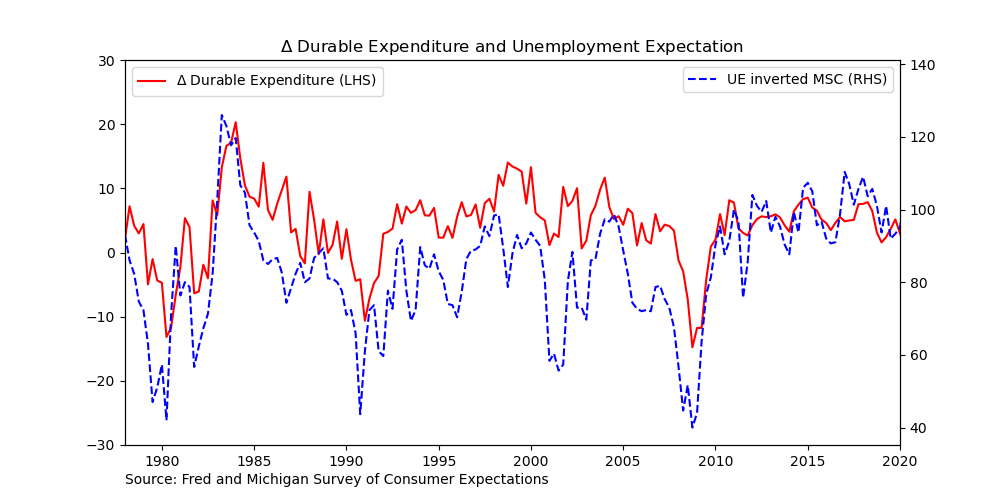
\includegraphics[width = 0.8\textwidth]{\FigDir/dur_vs_exp_emp.png}
	%\caption{Durable Expenditure and Expected Unemployment Rate} \label{fig:dur_vs_exp_emp}
%\end{figure}

\onlyinsubfile{% Allows two (optional) supplements to hard-wired \texname.bib bibfile:
% system.bib is a default bibfile that supplies anything missing elsewhere
% Add-Refs.bib is an override bibfile that supplants anything in \texfile.bib or system.bib
\provideboolean{AddRefsExists}
\provideboolean{systemExists}
\provideboolean{BothExist}
\provideboolean{NeitherExists}
\setboolean{BothExist}{true}
\setboolean{NeitherExists}{true}

\IfFileExists{\econtexRoot/Add-Refs.bib}{
  % then
  \typeout{References in Add-Refs.bib will take precedence over those elsewhere}
  \setboolean{AddRefsExists}{true}
  \setboolean{NeitherExists}{false} % Default is true
}{
  % else
  \setboolean{AddRefsExists}{false} % No added refs exist so defaults will be used
  \setboolean{BothExist}{false}     % Default is that Add-Refs and system.bib both exist
}

% Deal with case where system.bib is found by kpsewhich
\IfFileExists{/usr/local/texlive/texmf-local/bibtex/bib/system.bib}{
  % then
  \typeout{References in system.bib will be used for items not found elsewhere}
  \setboolean{systemExists}{true}
  \setboolean{NeitherExists}{false}
}{
  % else
  \typeout{Found no system database file}
  \setboolean{systemExists}{false}
  \setboolean{BothExist}{false}
}

\ifthenelse{\boolean{showPageHead}}{ %then
  \clearpairofpagestyles % No header for references pages
  }{} % No head has been set to clear

\ifthenelse{\boolean{BothExist}}{
  % then use both
  \typeout{bibliography{\econtexRoot/Add-Refs,\econtexRoot/\texname,system}}
  \bibliography{\econtexRoot/Add-Refs,\econtexRoot/\texname,system}
  % else both do not exist
}{ % maybe neither does?
  \ifthenelse{\boolean{NeitherExists}}{
    \typeout{bibliography{\texname}}
    \bibliography{\texname}}{
    % no -- at least one exists
    \ifthenelse{\boolean{AddRefsExists}}{
      \typeout{bibliography{\econtexRoot/Add-Refs,\econtexRoot/\texname}}
      \bibliography{\econtexRoot/Add-Refs,\econtexRoot/\texname}}{
      \typeout{bibliography{\econtexRoot/\texname,system}}
      \bibliography{        \econtexRoot/\texname,system}}
  } % end of picking the one that exists
} % end of testing whether neither exists
}

\ifthenelse{\boolean{Web}}{}{
  \onlyinsubfile{\captionsetup[figure]{list=no}}
  \onlyinsubfile{\captionsetup[table]{list=no}}
  \end{document}	\endinput
}

